\chapter{Kotlin/Native in de praktijk}
\label{ch:praktisch}
In dit hoofdstuk zal er praktisch een Kotlin/Native project worden opgebouwd. De bedoeling is om aan de hand van een voorbeeld de volledige werking uit te leggen. In dit voorbeeld zal er een simpele applicatie gebouwd worden, gericht op Android en iOS, waarbij gebruikers een shopping cart kunnen aanmaken, producten kunnen bekijken en toevoegen aan de shopping cart en kunnen bekijken welke producten reeds in hun winkelmandje aanwezig zijn. Het volledige project is te vinden op https://github.com/Iliasvw/kotlin-native-example.

\section{Domeinmodel}
\label{sec:domeinmodel}
Aangezien het doel van Kotlin/Native het delen van domeinlogica is, is het handig om op voorhand na te denken over het domeinmodel. Welke klassen zijn er nodig, welke attributen en methodes moeten deze klassen hebben, is er eventueel in implementatie van klassen tussen Android en iOS? Een domeinmodel geeft ook een duidelijk overzicht over de logica van de applicatie. Zie figuur \ref{fig:domeinmodel-kn} om het domeinmodel te bekijken van deze voorbeeldapplicatie. 

Het domeinmodel beschikt over drie klassen: 
\begin{itemize}
	\item De klasse Cart stelt het winkelmandje voor. Deze beschikt over een naam en kan nul, één of meerdere CartLines bevatten. De klasse heeft een constructor die een naam verwacht en methodes om een CartLine toe te voegen, alle CartLines op te vragen, de totale prijs van het winkelmandje te berekenen en een CartLine te verwijderen van het winkelmandje.
	
	\item Een CartLine object heeft een product en quantity (hoeveelheid) attribuut. Deze klasse beschikt over een constructor die twee parameters verwacht, die tevens onze attributen zijn. Deze is ook voorzien van twee getters, om de attributen op te vragen (aangezien deze private zijn) en een methode om de kostprijs van deze CartLine te berekenen.
	
	\item De product klasse is de klasse die per platform wordt geïmplementeerd. Deze klasse wordt dus als expect gedeclareerd en beschikt over drie expect methodes om de attributen van de klasse op te vragen. Per platform, in dit voorbeeld zal dit Android en iOS zijn, wordt er een implementatie voorzien van deze klasse. Deze actual klassen hebben elk een name, price, description en productImage en een implementatie van de methodes van de expect Product klasse. Het type van de productImage verschilt per platform.
\end{itemize}

\begin{figure} [ht]
	\centering
	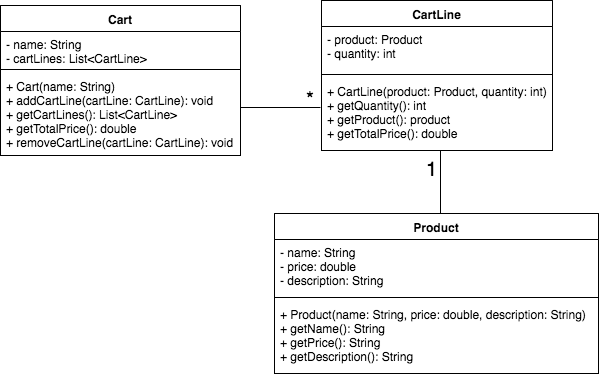
\includegraphics[width=0.95\textwidth]{img/domeinmodel.png}
	\caption{Klassendiagram domeinlogica}
	\label{fig:domeinmodel-kn}
\end{figure}

\section{Requirements}
Om gebruik te kunnen maken van Kotlin/Native voor het ontwikkelen van cross-platform applicaties (Android en iOS), zijn er enkele vereisten:
\begin{itemize}
	\item \textbf{Android studio} voor het ontwikkelen van de Android applicatie.
	\item \textbf{Xcode} voor het ontwikkelen van de iOS applicatie (toestel met MacOS is vereist).
	\item \textbf{IntelliJ IDEA} (optioneel) voor het opzetten van het project. Dit kan eventueel met een andere IDEA, die gradle projecten ondersteunt, worden opgezet.
	\item \textbf{Gradle} om gebruik te kunnen maken van de Kotlin/Native compiler en plugin. Deze wordt automatisch geïnstalleerd bij het instellen van IntelliJ IDEA of Android Studio.
\end{itemize}

\section{Wat is gradle?}
Gradle is een build systeem. Het combineert de beste features van vele andere build systemen en combineert deze tot één systeem. Het is een op JVM gebaseerd build systeem wat betekent dat er eigen geschreven Java scripts kunnen worden gebruikt. 

Android Studio maakt gebruikt van Gradle. Waarom maakt Google gebruikt van Gradle? Google zag Gradle als een zeer geavanceerd build systeem en realiseerde dat er eigen geschreven build scripts gebruikt kunnen worden met zo goed als geen leercurve. Het was ook niet nodig om een andere programmeertaal aan te leren aangezien er scripts kunnen worden geschreven in Java. Hierdoor is de Gradle plugin toegevoegd aan Android Studio \autocite{GoogleGradle}.

\section{Stap 1: project initiatie}
De eerste stap in het ontwikkelen van een Kotlin/Native project is het maken van een nieuwe map op een gewenste locatie op de harde schijf van de computer. Hierin zal er een eerste bestand worden aangemaakt: \textbf{build.gradle}.

\begin{lstlisting}
subprojects {
 buildscript {
  ext.kotlin_version = '1.2.31'
  ext.kotlin_native_version = '0.6.2'
		
  repositories {
   jcenter()
   google()
   maven { url "http://kotlin.bintray.com/kotlinx" }
   maven { url "https://plugins.gradle.org/m2/" }
   maven { url "https://dl.bintray.com/jetbrains/ kotlin-native-dependencies" }
  }

  dependencies {
   classpath "org.jetbrains.kotlin:kotlin-gradle-plugin: $kotlin_version"
   classpath 'com.android.tools.build:gradle:3.0.1'
   classpath "org.jetbrains.kotlin:kotlin-native-gradle-plugin: $kotlin_native_version"
  }
 }
	
 group 'ilias.vw'
 version '1.0-SNAPSHOT'
	
 repositories {
  jcenter()
  maven { url "http://kotlin.bintray.com/kotlinx" }
 }
	
 tasks.withType(Test) {
  testLogging {
   showStandardStreams = true
   events "passed", "failed"
  }
 }
}
\end{lstlisting}
Hieronder wordt de inhoud van het build.gradle bestand besproken.
\subsection{Versies}
Bovenaan wordt er aangegeven welke versie van Kotlin en Kotlin/Native er gebruikt zal worden voor de opzet van dit project. Dit zijn beide de nieuwste versies. Opgelet, het is niet altijd vanzelfsprekend om de laatste versie van Kotlin/Native te gebruiken. Er wordt voortdurend gewerkt aan Kotlin en Kotlin/Native en nieuwe dingen worden continu gepusht op de GitHub repository. Het kan al eens gebeuren dat sommige features niet altijd even goed werken, wat voor problemen kan zorgen bij de ontwikkeling van de applicatie. Bij twijfels, neem een minder recente versie van de Kotlin/Native plugin.

\subsection{Repositories}
In de repositories tag worden de juiste repositories gelinkt:
\begin{itemize}
	\item \textbf{Kotlinx} bevat alle coroutines\footnote{Programmaonderdelen die asynchroon programmeren vergemakkelijken door gecompliceerde logica in bibliotheken te steken} die Kotlin kan gebruiken.
	\item \textbf{Gradle}
	\item \textbf{Kotlin-native-dependencies} stelt alle dependencies, die Kotlin/Native nodig heeft, ter beschikking.
\end{itemize}

\subsection{Dependencies}
In de dependencies tag worden de juiste dependencies gelinkt:
\begin{itemize}
	\item \textbf{Kotlin-gradle} laadt de Kotlin-gradle plugin met de versie van Kotlin die wordt aangegeven bovenaan het build script. Deze plugin zorgt voor het compileren van Kotlin bronnen en modules.
	\item \textbf{Android build tools} is nodig voor het bouwen van de Android applicatie.
	\item \textbf{Kotlin-native-gradle-plugin} is de Kotlin/Native plugin die gebruikt zal worden om te zorgen voor een cross-platform applicatie.
\end{itemize}

\subsection{Overige informatie}
\label{sec:overige}
\begin{itemize}
	\item \textbf{Group} stelt het groupId van het project in.
	\item \textbf{Version} geeft de versie van het project weer.
	\item \textbf{testLogging} wordt gebruikt voor het uitvoeren van de testen.
\end{itemize}

\subsection{Build map}
Voor elke map die een build.gradle bestand bevat zal er automatisch een build folder worden gegenereerd. De build map bevat alle gecompileerde bestanden, van een bepaalde map, die gegenereerd worden door Kotlin/Native en deze worden bij iedere gradle run en/of build aangemaakt.

\section{Stap 2: project structuur}
Nadat het build.gradle bestand aangemaakt is, is het de bedoeling om via IntelliJ IDEA het gradle bestand te importeren. Zie figuur \ref{fig:stap2-import}. IntelliJ zal een dialoogvenster openen, waarbij het build.gradle bestand moet worden geopend. De IDE zal hierna het build.gradle bestand uitvoeren en het genereert enkele bestanden.

\begin{figure} [ht]
	\centering
	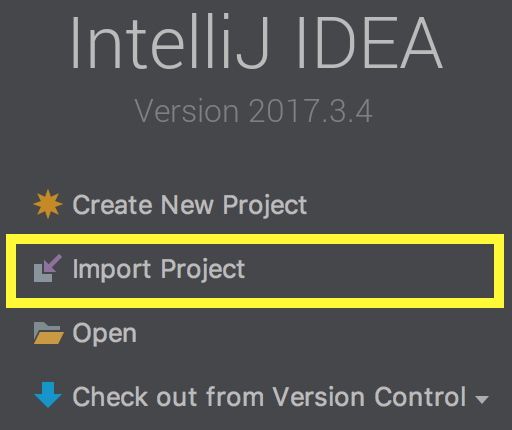
\includegraphics[width=0.60\textwidth]{img/stap2-import.png}
	\caption{Importeren van een project}
	\label{fig:stap2-import}
\end{figure}

In de huidige versie van Kotlin/Native worden de overige mappen nog niet automatisch aangemaakt. Alle andere mappen, die te zien zijn in figuur \ref{fig:knstructuur} moeten handmatig aangemaakt worden. Deze mappenstructuur zal geleidelijk aan opgebouwd worden naargelang de stappen vorderen.

\section{Stap 3: Common map }
In de common map wordt alle gemeenschappelijke code geschreven. De inhoud van deze map moet aan een bepaalde structuur voldoen, zie figuur \ref{fig:stap3-common}. In sectie \ref{sec:gradlecommon} wordt uitgelegd waarom deze structuur zo belangrijk is.

\begin{figure} [ht]
	\centering
	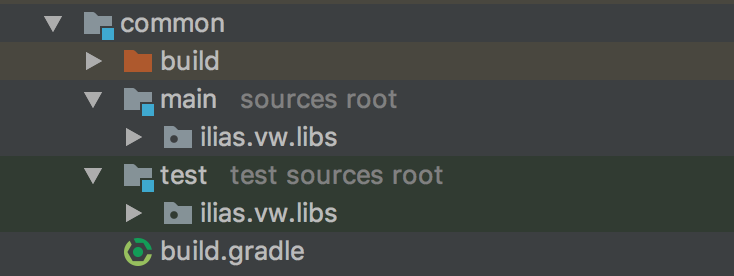
\includegraphics[width=0.60\textwidth]{img/stap3-common.png}
	\caption{Common module structuur}
	\label{fig:stap3-common}
\end{figure}

\subsection{Main en test map}
\label{sec:maintestcommon}
Zoals te zien is op figuur \ref{fig:stap3-common} heeft zowel de main als test map enkele subpackages. Deze beginnen met het groupId dat ingesteld is in sectie \ref{sec:overige} met daarin nog eens een 'libs' package. De naam van deze 'libs' package is vrij te kiezen, maar in dit voorbeeldproject wordt altijd 'libs' gebruikt.

De main map zal alle gemeenschappelijke klassen bevatten. Dit zijn zowel de klassen die expect gedeclareerd zijn als de klassen die een concrete implementatie hebben. Zie sectie \ref{sec:expectandactual} voor uitleg over het expect keyword.

De test map zal alle gemeenschappelijke test klassen bevatten, gebruikmakend van de klassen in de main map.

\subsection{Build.gradle}
\label{sec:gradlecommon}
Natuurlijk moet de common module ook gecompileerd worden door Kotlin/Native. Hiervoor is er een build.gradle nodig.

\begin{lstlisting}
apply plugin: 'kotlin-platform-common'

sourceSets {
 main.kotlin.srcDirs += 'main/'
 test.kotlin.srcDirs += 'test/'
}

dependencies {
 compile "org.jetbrains.kotlin:kotlin-stdlib-common:$kotlin_version"
 testCompile "org.jetbrains.kotlin:kotlin-test-annotations-common: $kotlin_version"
 testCompile "org.jetbrains.kotlin:kotlin-test-common:$kotlin_version"
}
\end{lstlisting}
De bovenste regel in de build.gradle geeft aan dat de kotlin-platform-common plugin gebruikt zal worden. Deze zal verantwoordelijk zijn voor het compileren en delen van alle gemeenschappelijke code over de verschillende platformen.

Er worden ook twee sourceSets toegevoegd. SourceSets vertegenwoordigen een logische groep van Java/Kotlin bronnen. Kotlin/Native zal steeds zoeken naar code in de map src/kotlin/main of src/kotlin/test, maar hier geven we aan dat code te vinden is in de main en test map en dus niet onder een src/kotlin/ map.

Tenslotte worden er drie dependencies toegevoegd. De stdlib is verantwoordelijk verlenen van toegang tot de standaard bibliotheek van Kotlin. Hierdoor hebben we toegang tot collections, streams, annotations en nog veel meer. Er worden nog twee test dependencies toegevoegd, één verantwoordelijk voor de annotations, de andere voor het opstellen en uitvoeren van de testen, zie sectie \ref{sec:testing} voor meer informatie over het opstellen van testen.

\section{Common code}
Uitwerking van de common code van de voorbeeldapplicatie.
\subsection{Cart}
Implementatie van de Cart klasse in de common module. Dit is een doodnormale Kotlin klasse en heeft weinig Kotlin/Native specifiek.
\begin{lstlisting}
package ilias.vw.libs
	
class Cart constructor(name: String) {
 var name: String = name
 private var cartLines: List<CartLine> = mutableListOf()
	
 fun getCartLines(): List<CartLine> {
  return this.cartLines
 }
	
 fun addCartLine(cartLine: CartLine) {
  for (item in cartLines) {
   if (item.getProduct().getName() == cartLine.getProduct().getName()) {
    item.add(cartLine.getQuantity())
    return
   }
  }
  this.cartLines += cartLine
 }
	
 fun getTotalPrice(): Double {
  var totalPrice = 0.0
	
  for (line in cartLines) {
   totalPrice += line.getTotalPrice()
  }
	
  return totalPrice
 }
	
 fun removeCartLine(cartLine: CartLine) {
  this.cartLines -= cartLine
 }
}
\end{lstlisting}

\subsection{CartLine}
Implementatie van de CartLine klasse in de common module. Ook deze klasse heeft niks Kotlin/Native specifiek.
\begin{lstlisting}
package ilias.vw.libs

class CartLine {
 private val product: Product
 private val quantity: Int

 constructor(product: Product, quantity: Int) {
  this.product = product
  this.quantity = quantity
 }

 fun getProduct(): Product {
  return this.product
 }

 fun getQuantity(): Int {
  return this.quantity
 }

 fun getTotalPrice(): Double {
  return product.getPrice() * quantity
 }
}
\end{lstlisting}

\subsection{Product}
De product klasse is een expect klasse. Dit wil zeggen dat we voor iedere platform een andere implementatie hebben voor deze klasse. Maar voor iedere platform verwachten we wel dat deze de getName, getPrice en getDescription methodes heeft.

\begin{lstlisting}
package ilias.vw.libs

expect class {
 fun getName(): String
 fun getPrice(): Double
 fun getDescription(): String
}
\end{lstlisting}

\section{Stap 4: platforms folder}
De platform folder bevat enkele subfolders, één subfolder per platform waarvoor men wenst te ontwikkelen. Bij dit voorbeeld zijn er dus twee subfolders aanwezig, namelijk Android en iOS. Zie figuur \ref{fig:stap4-structuur}. Per submap, hebben we opnieuw twee submappen, namelijk main en test. Net zoals bij de common map. 

\begin{figure} [ht]
	\centering
	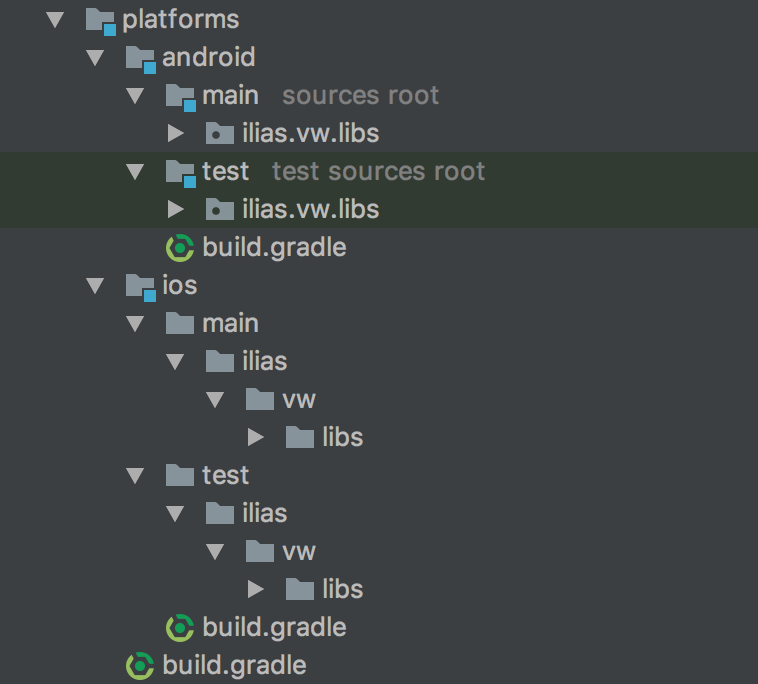
\includegraphics[width=0.60\textwidth]{img/stap4-structuur.png}
	\caption{Platforms module structuur}
	\label{fig:stap4-structuur}
\end{figure}

Zowel de main en test map bevatten elk nog een map. Bij Android is dit een package die begint met het groupId, zie sectie \ref{sec:overige}, en eindigt met een willekeurige naam. In dit voorbeeld is dit opnieuw 'libs'. Dit dient identiek te zijn aan de naam van de package gekozen in de common map, zie sectie \ref{sec:maintestcommon}. In het geval van iOS zijn dit geen packages maar eerder een mappenstructuur.

\subsection{Platforms android map}
\subsubsection{Build.gradle}
\begin{lstlisting}
apply plugin: 'kotlin-platform-jvm'

repositories {
 jcenter()
 maven { url "http://kotlin.bintray.com/kotlinx" }
}

sourceSets {
 main.kotlin.srcDirs += 'main/'
 test.kotlin.srcDirs += 'test/'
}

dependencies {
 compile "org.jetbrains.kotlin:kotlin-stdlib:$kotlin_version"
 expectedBy project(":common")

 testCompile "junit:junit:4.12"
 testCompile "org.jetbrains.kotlin:kotlin-test-junit: $kotlin_version"
 testCompile "org.jetbrains.kotlin:kotlin-test:$kotlin_version"
}
\end{lstlisting}

In deze build.gradle wordt er gebruik gemaakt van de kotlin-platform-jvm plugin. Android applicaties maken nog steeds gebruik van de JVM en dus ook deze android applicatie. De JVM voert een aantal noodzakelijk taken uit die ook Kotlin nodig heeft in Android applicaties, zie sectie \ref{sec:jvm} voor meer uitleg over de JVM. De sourceSets worden ingesteld. Tenslotte worden alle dependencies geladen en wordt er aangegeven dat de common module verwacht wordt die code bevat.

\subsubsection{Platformspecifieke code}
De platformspecifieke code voor Android. De klasse product wordt voorzien van een afbeelding en aangezien drawables in Android gemapt worden naar een integerwaarde, wordt er een getal ingevuld in de constructor. De naam van het product wordt teruggeven met prefix 'Android'.
\begin{lstlisting}
package ilias.vw.libs

import java.io.Serializable

actual class Product: Serializable {
 private val name: String
 private val price: Double
 private val description: String
 private val productImage: Int

 actual constructor(name: String, price: Double, 
		description: String, productImage: Int) {
  this.name = name;
  this.price = price
  this.description = description
  this.productImage = productImage
 }

 actual fun getName(): String {
  return "Android: $name"
 }

 actual fun getPrice(): Double {
  return this.price
 }

 actual fun getDescription(): String {
  return this.description
 }

 actual fun getProductImage(): Int {
  return this.productImage
 }
}
\end{lstlisting}

\subsection{Platforms ios map}
\subsubsection{Build.gradle}
\label{sec:ios-build-gradle}
\begin{lstlisting}
apply plugin: 'konan'

konanArtifacts {
 framework('SharediOS', targets: ['iphone', 'iphone_sim']){
  enableDebug true
  enableMultiplatform true

  srcDir 'main'
 }

 library('test-library') {
  enableMultiplatform true
  srcDir 'main'
 }

 program('shared-ios-test') {
  srcDir 'test'
  commonSourceSet 'test'
  extraOpts '-tr'
  libraries {
   artifact 'test-library'
  }
 }
}

dependencies {
 expectedBy project(':common')
}
\end{lstlisting}

Zoals reeds te lezen is in sectie \ref{sec:use-ios-code} zal Kotlin/Native alle Kotlin code compileren naar een iOS framework. In de build.gradle wordt de naam van het framework en de toestellen (iPhone en iPhone simulators) dat men wenst te ondersteunen ingesteld.

De main map wordt als source directory ingesteld. Om ervoor te zorgen dat op iOS ook de testen kunnen worden uitgevoerd, wordt de main map ingesteld als bron van klassen die gebruikt kunnen worden voor alle testen en de test map wordt ingesteld als bron waar alle testen zijn gelokaliseerd.

Tenslotte wordt er opnieuw aangegeven dat er een common module wordt verwacht die alle gemeenschappelijke code bevat.

\subsubsection{Platformspecifieke code}
De platformspecifieke code voor iOS. In iOS is er de mogelijkheid om afbeeldingen in te laden aan de hand van de naam van de imageset. Daardoor heeft de constructor een productImage die van het type String is. De naam van het product wordt teruggegeven met prefix 'iOS'.
\begin{lstlisting}
package ilias.vw.libs

actual class Product {
 private val name: String
 private val price: Double
 private val description: String
 private val productImage: String

 actual constructor(name: String, price: Double, 
		description: String, productImage: String) {
  this.name = name;
  this.price = price
  this.description = description
  this.productImage = productImage
 }

 actual fun getName(): String {
  return "iOS: $name"
 }

 actual fun getPrice(): Double {
  return this.price
 }

 actual fun getDescription(): String {
  return this.description
 }

 fun getProductImage(): String {
  return this.productImage
 }
}
\end{lstlisting}

\section{Stap 5: Android map}
In de android map is het de bedoeling om via Android Studio een nieuw project aan te maken. Bij het aanmaken van het project in Android Studio kan de locatie van het project worden opgeven. Deze locatie moet zodanig ingesteld zijn dat het Android project een submap is van het Kotlin/Native project en waardoor het geïntegreerd zal worden in dit project.

\subsection{settings.gradle}
Voor we gebruik kunnen maken van de Kotlin klassen, moeten er eerst nog enkele wijzigingen gebeuren in de settings.gradle van het Android project. De settings.gradle wordt vervangen door onderstaande code:

\begin{lstlisting}
include ':app'

include ':common'
project(":common").projectDir = new File("../common")

include ':platforms-android'
project(":platforms-android").projectDir = new File("../platforms/android")
\end{lstlisting}

Via de settings.gradle wordt er aangegeven om de common en platforms-android modules te includen in het project. Hierdoor worden de common en platformspecifieke Android modules geïntegreerd in het Android project.

\subsection{build.gradle}
Tenslotte moet er nog een kleine wijziging doorgevoerd worden in de build.gradle van het Android project. In de dependencies tag moet er enkel en alleen volgende lijn toegevoegd worden in de dependencies tag:

\begin{lstlisting}
implementation project(':platforms-android')
\end{lstlisting}

Hiermee wordt er aangegeven dat de specifieke Android implementatie te vinden is in platforms-android, waarvan de locatie is opgegeven in de settings.gradle. Vanaf nu kan er gebruik gemaakt worden van de klassen in de common module en de platformspecifieke Android module.

\section{Stap 6: iOS map}
\label{sec:ios-stap6}
Net zoals bij de android map, is het de bedoeling om via Xcode een nieuw Xcode project aan te maken dat ook een submap is van het Kotlin/Native project. Men kan zowel kiezen voor een Objective-C als Swift project aangezien het gecompileerde iOS framework zowel in beide projecten kan gebruikt worden.

\subsection{Gebruiken van het SharediOS framework}
Vooraleer men in Xcode kan gebruik maken van het SharediOS framework, moeten er een aantal dingen aangepast worden in de build phases van het project. Uit figuur \ref{fig:stap6-phases} kan worden afgeleid dat de build phases zijn aangepast. Volgende build phase moet worden toegevoegd: Compile Kotlin Native to iOS framework.
\begin{figure} [ht]
	\centering
	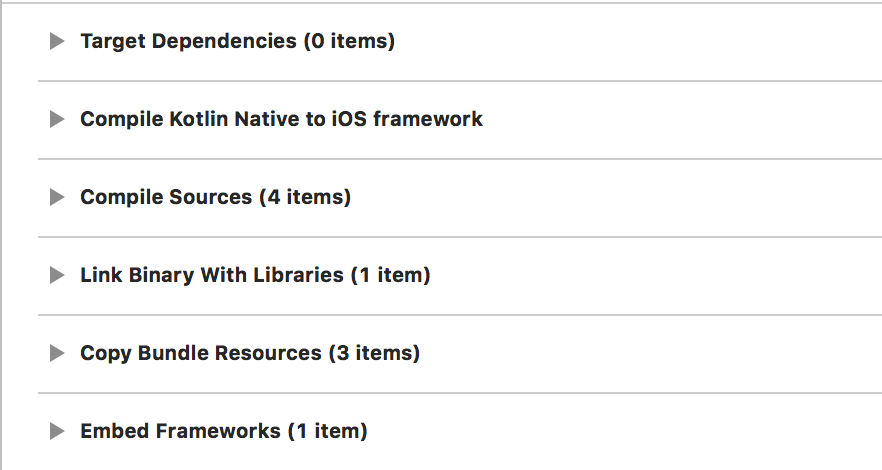
\includegraphics[width=0.75\textwidth]{img/stap6-phases.png}
	\caption{iOS build phases}
	\label{fig:stap6-phases}
\end{figure}

In deze nieuwe build phase moet er een script, afkomstig van \textcite{AlbertGao}, worden toegevoegd: 
\begin{lstlisting}
case "$PLATFORM_NAME" in iphoneos)
NAME=iphone;;
iphonesimulator)
NAME=iphone_sim;;
*)
echo "Unknown platform: $PLATFORN_NAME"
exit 1;;
esac

"$SRCROOT/../gradlew" -p "$SRCROOT/../platforms/ios" "build"
rm -rf "$SRCROOT/build/"
mkdir "$SRCROOT/build/"
cp -a "$SRCROOT/../platforms/ios/build/konan/bin/$NAME/" "$SRCROOT/build/"
\end{lstlisting}

Bij iedere gradle build van het Kotlin/Native project zal de build.gradle in de platforms/ios map ervoor zorgen dat de Kotlin code omgezet wordt naar een iOS framework. Dit framework vindt men terug in een submap van de build map (platforms/ios/build/). Zie figuur \ref{fig:stap6-build}. Er wordt dus zowel voor een echt toestel (iphone map) als voor een simulator (iphone\char`_sim map) een framework gegenereerd. Dit wordt gedaan omdat beiden op verschillende architecturen worden uitgevoerd.

\begin{figure} [ht]
	\centering
	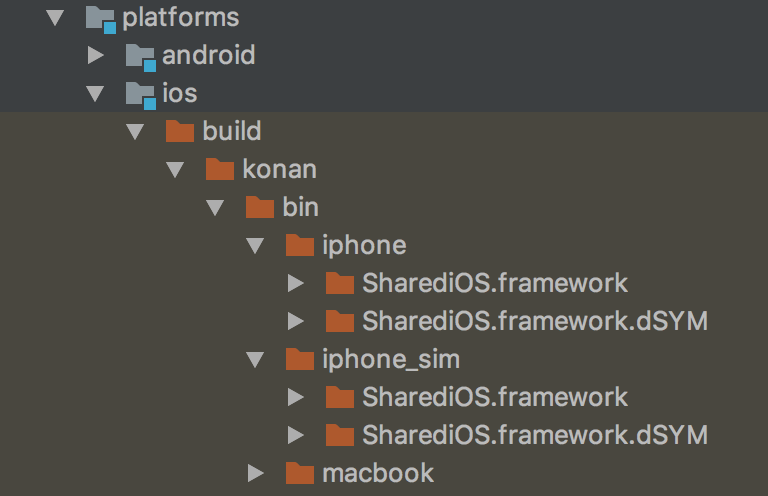
\includegraphics[width=0.60\textwidth]{img/stap6-build.png}
	\caption{iOS build map}
	\label{fig:stap6-build}
\end{figure}

In bovenstaand build phase script wordt gekeken welk type toestel er wordt gebruikt, een echte iPhone of een simulator. Daarna zal het juiste framework gekopieerd worden naar de build folder in de map van het Xcode project. Bij iedere build en/of run van het Xcode project zal bovenstaand script worden uitgevoerd. Dit zal ervoor zorgen dat steeds het laatst gegenereerde framework gebruikt zal worden door het Xcode project.

Tenslotte zal het framework nog in de build phases 'Link Binary With Libraries' en 'Embed Frameworks' moeten worden toegevoegd. Hierbij wordt er gelinkt naar het gekopieerde framework in de build folder van het Xcode project.

\section{Aanspreken van code}
\subsection{Android}
Om gebruik te kunnen maken van de Kotlin code in het Android project moet men simpelweg volgende import toevoegen om alle klassen te kunnen gebruiken: 

\begin{lstlisting}
import ilias.vw.libs.*
\end{lstlisting}

\subsection{iOS}
Om gebruik te kunnen maken van het SharediOS framework in de ViewControllers moet het framework worden geïmporteerd door bovenaan in de ViewController volgende lijn toe te voegen:

\begin{lstlisting}
import SharediOS
\end{lstlisting}

Het aanmaken van een object in iOS is nu heel simpel geworden. Zoals te zien is in onderstaande code heeft Kotlin/Native een prefix gegeven aan de klassen. Kotlin/Native zal steeds de hoofdletters uit de naam van het framework filteren, dat gekozen wordt in de build.gradle van de iOS folder, zie sectie \ref{sec:ios-build-gradle}. Stel dat het framework KotlinNativeFramework heet, dan zal de prefix KNF zijn en zal de product klasse KNFProduct heten. In dit voorbeeld heet het gecompileerde iOS framework SharediOS, waardoor de prefix SOS is.

\begin{lstlisting}
var product: SOSProduct = SOSProduct(name: "Playstation 4", price: 399.95, description: "Playstation 4 gaming console", productImage: "ps4")
\end{lstlisting}

\section{User interfaces}
De user interface moet dus per platform opgebouwd worden. Er is geen manier om één user interface te ontwikkelen voor beide platformen zoals bijvoorbeeld bij React/Native of Ionic. Dit kan zowel positief als negatief zijn. Het vraagt dubbel zoveel werk maar het geeft wel de mogelijkheid om verschillende accenten te leggen in de user interface per platform.

\section{Testen}
\label{sec:testing}
Een essentieel deel van object-oriented programming is het testen van de code. In het Kotlin/Native framework is het mogelijk om de aangemaakte klassen te testen. Zo is er de mogelijkheid om in de common map en per platform een test map toe te voegen. Een voorbeeld van een testklasse:

\begin{lstlisting}
package ilias.vw.libs

import kotlin.test.*

class TestSampleCommon {
 @Test
 fun testCheckChartName() {
  val sample = Cart("test")
  val name = sample.name
  assertEquals(name, "test")
 }
}

\end{lstlisting}

Hierbij wordt er een cart aangemaakt met een naam 'test'. Daarna wordt de naam terug opgevraagd en wordt er gekeken of de naam die we initieel hebben meegegeven effectief gelijk is aan 'test'.

Aangezien er per platform, platformspecifieke code geschreven kan worden is het belangrijk om deze code ook te kunnen testen. Er kan naargelang dat de code per platform verschilt, verschillende testcode geschreven worden in de test map van het platform. Dit zorgt ervoor dat er geen ongeteste code in het project geraakt wat eventueel bugs kan bevatten. 

Een voorbeeld voor deze proof-of-concept: er kan voor de ios test gecheckt worden of de naam van het product begint met de prefix 'iOS' en voor Android kan er gecheckt worden of deze naam start met prefix 'Android'.

\section{Huidige mogelijkheden}
Zoals uit de proof-of-concept af te leiden is, is het reeds mogelijk om Kotlin/Native te gebruiken om een cross-platform applicatie te ontwikkelen. Aan de hand van de Kotlin/Native Gradle plugin is het mogelijk om niet alleen voor Android te ontwikkelen maar ook voor iOS. Cross-platform heeft bij Kotlin/Native niet dezelfde betekenis als bij een framework zoals React/Native. Het doel van Kotlin/Native is dus het delen van domeinlogica en deze hergebruiken over de verschillende te ondersteunen platformen. In deze vroege versie (0.6) van Kotlin/Native is het reeds mogelijk om dit te doen, maar de mogelijkheden blijven beperkt. Indien de applicatie geen speciale iOS bibliotheken nodig heeft, is er geen probleem.

Een ander belangrijk luik dat Kotlin/Native reeds ondersteunt is het aanmaken van testen voor de geschreven domeinlogica. Testen zijn en blijven een belangrijke onderdeel van object-oriented programming.

\section{Beperkingen}
Aangezien er nog geen officiële versie van Kotlin/Native is vrijgegeven is het logisch dat de mogelijkheden nog zeer beperkt zijn. 

Er kan voor de platformspecifieke iOS code geen iOS specifieke bibliotheken gebruikt worden. In deze proof-of-concept was het de bedoeling om de shopping cart in zowel Android als iOS te cachen. In iOS moet het object dat gecached moet worden voldoen aan een bepaalde protocol, namelijk Codable. Kotlin/Native heeft geen kennis van deze protocollen waardoor het dus niet mogelijk is om het object te cachen in iOS. Voor Android kon dit wel, indien een bepaald object gecached moet worden volstaat het om deze klasse de interface Serializable te laten implementeren. Dit is niet mogelijk in de common module aangezien iOS het protocol Serializable niet kent. Dit is wel mogelijk in de platformspecifieke code van Android. Voor Android is het wel mogelijk om interfaces te implementeren maar dan moet de klasse in de common module expect worden gedeclareerd en moet de actual klasse, in de Android platforms map, deze interface implementeren. Dit is het geval bij het domeinmodel van deze proof-of-concept, zie figuur \ref{fig:domeinmodel-kn}.

Het aanspreken van hardware, zoals de Camera, via Kotlin/Native is (nog) niet mogelijk. Momenteel moet het openen van bijvoorbeeld de camera geprogrammeerd worden in het Android en Xcode project, er is (nog) geen manier om dit te doen in bijvoorbeeld de common module.

Het gebruik van expect en actual klassen is momenteel ook nog zeer beperkt. Indien er een bepaalde klasse expect wordt gedeclareerd is het verder niet mogelijk om methodes of attributen toe te voegen aan deze klasse die niet expect zijn. Momenteel kan dus een expect klasse enkel en alleen expect methodes bevatten.

\section{Proof-of-concept}
\label{sec:poc}
Hieronder zijn de screenshots van de schermen van de proof-of-concept te vinden, opgesplitst per platform (Android en iOS).
\newpage
\subsection{Android}
\begin{figure}[H]
	\centering
	\begin{subfigure}{.5\textwidth}
		\centering
		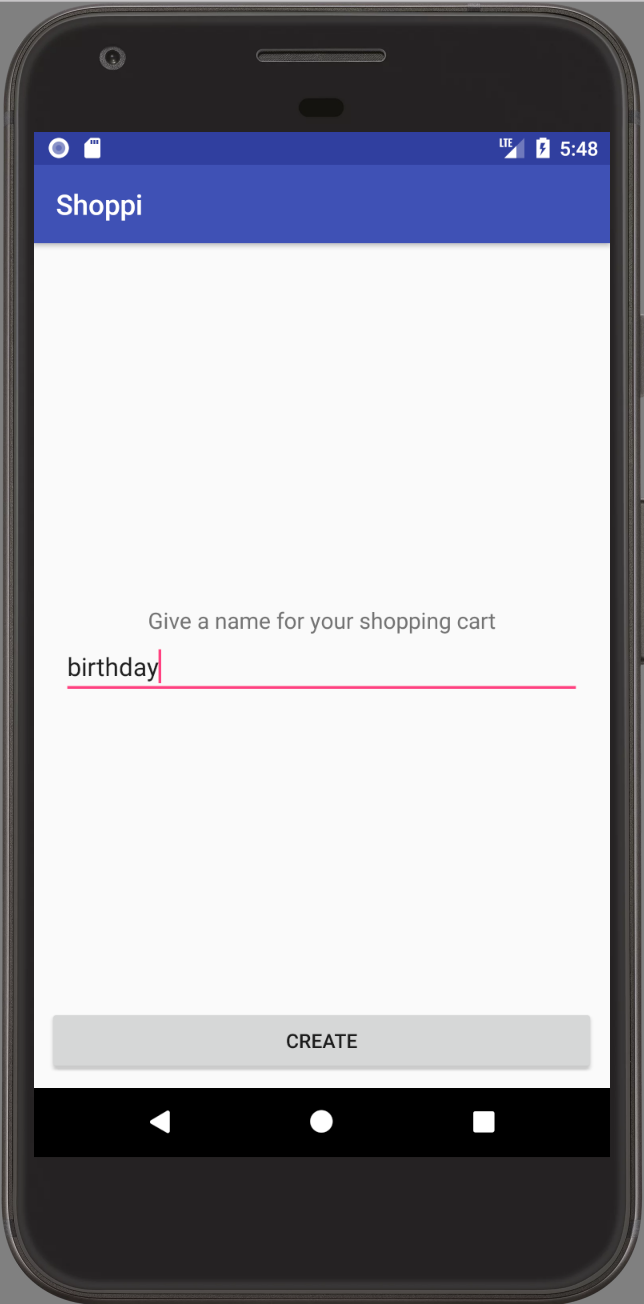
\includegraphics[width=0.65\linewidth]{img/poc/android/1.png}
		\caption{Aanmaken van een shopping cart}
	\end{subfigure}%
	\begin{subfigure}{.5\textwidth}
		\centering
		
\includegraphics[width=0.65\linewidth]{img/poc/android/2.png}
		\caption{Overzicht van producten}
		\label{fig:sub2}
	\end{subfigure}
\begin{subfigure}{.5\textwidth}
	\centering
	
\includegraphics[width=0.65\linewidth]{img/poc/android/3.png}
	\caption{Details van een product}
	\label{fig:sub1}
\end{subfigure}%
\begin{subfigure}{.5\textwidth}
	\centering
	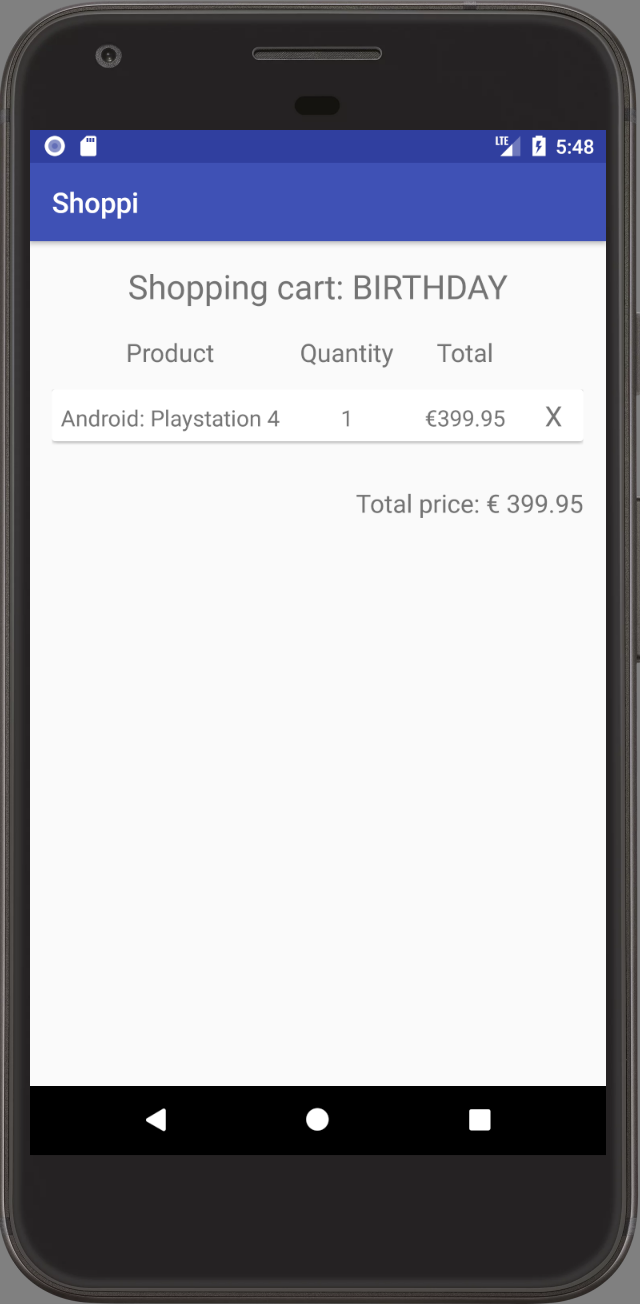
\includegraphics[width=0.65\linewidth]{img/poc/android/4.png}
	\caption{Overzicht winkelmand}
	\label{fig:sub2}
\end{subfigure}
	\caption{Screenshots Android}
	\label{fig:test}
\end{figure}

\subsection{iOS}
\begin{figure}[H]
	\centering
	\begin{subfigure}{.5\textwidth}
		\centering
		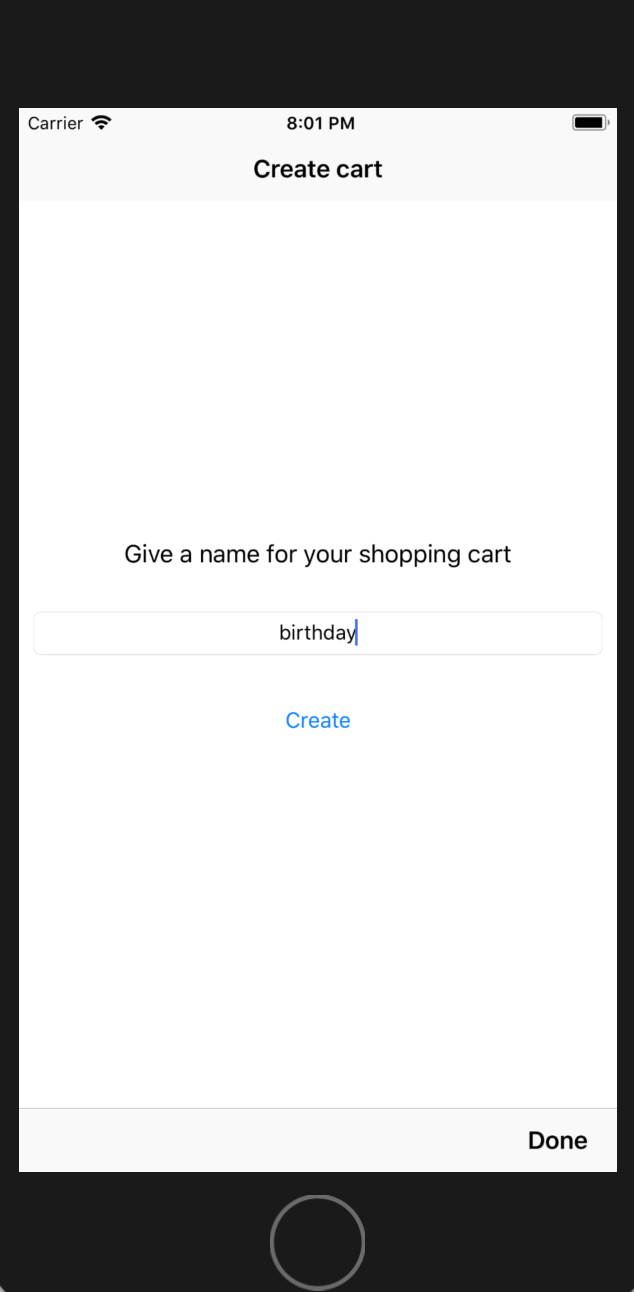
\includegraphics[width=0.65\linewidth]{img/poc/ios/1.png}
		\caption{Aanmaken van een shopping cart}
	\end{subfigure}%
	\begin{subfigure}{.5\textwidth}
		\centering
		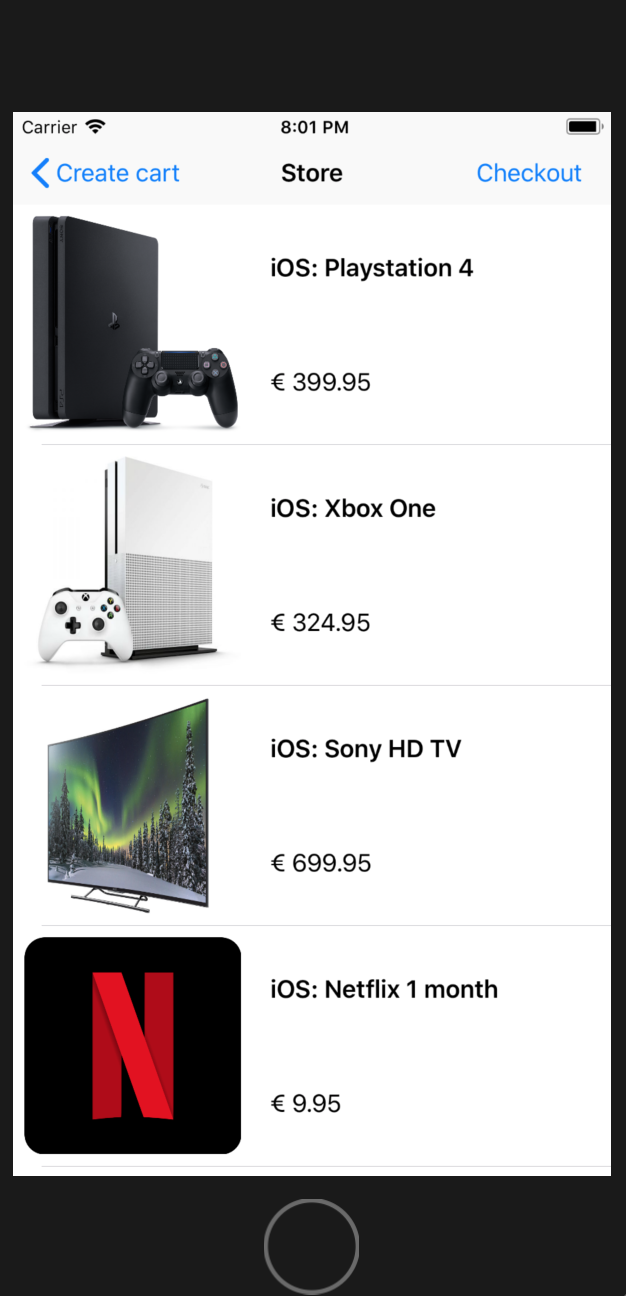
\includegraphics[width=0.65\linewidth]{img/poc/ios/2.png}
		\caption{Overzicht van producten}
		\label{fig:sub2}
	\end{subfigure}
	\begin{subfigure}{.5\textwidth}
		\centering
		
\includegraphics[width=0.65\linewidth]{img/poc/ios/3.png}
		\caption{Details van een product}
		\label{fig:sub1}
	\end{subfigure}%
	\begin{subfigure}{.5\textwidth}
		\centering
		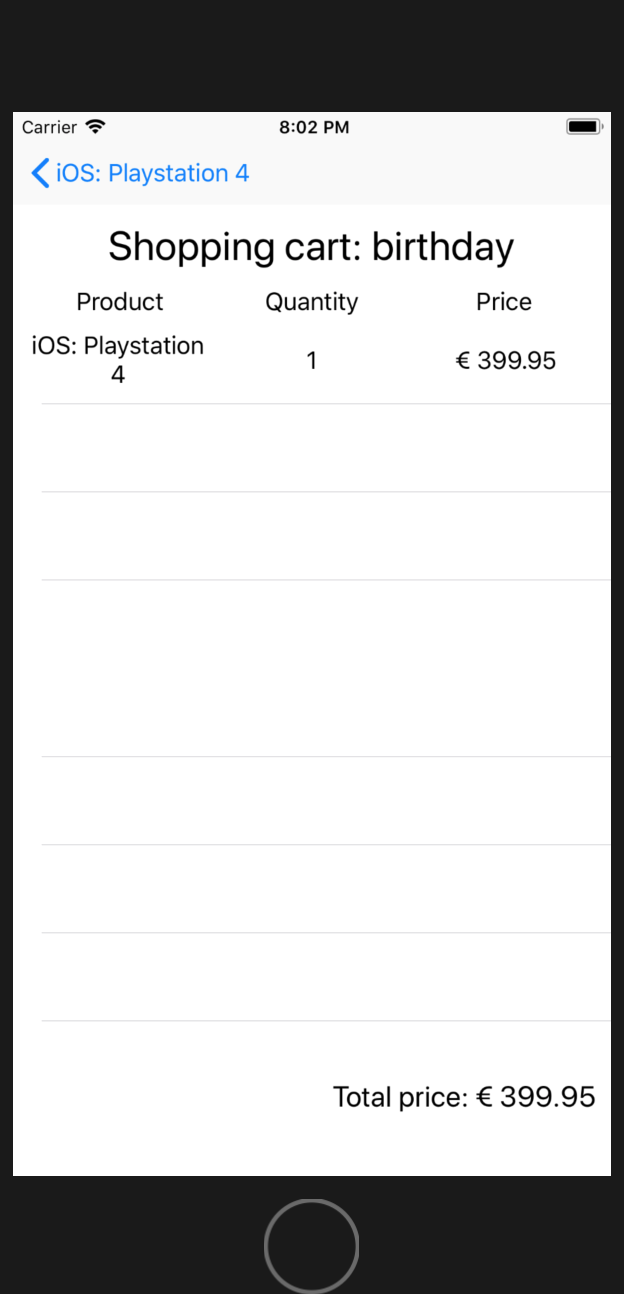
\includegraphics[width=0.65\linewidth]{img/poc/ios/4.png}
		\caption{Overzicht winkelmand}
		\label{fig:sub2}
	\end{subfigure}
	\caption{Screenshots iOS}
	\label{fig:test}
\end{figure}